\documentclass[tikz,convert={density=300,outext=.png}]{standalone}
\usetikzlibrary{arrows.meta,graphs}
\begin{document}
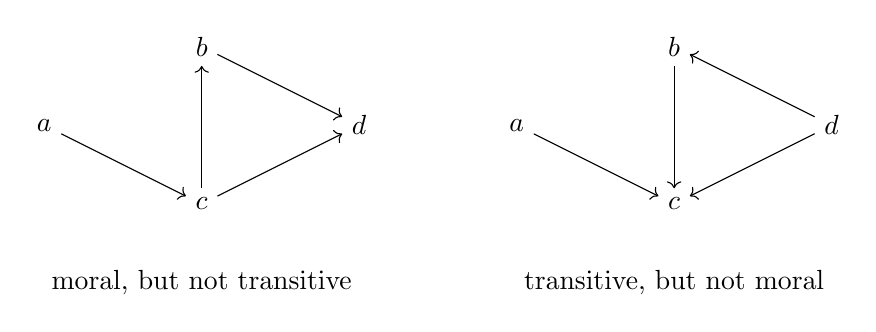
\begin{tikzpicture}
    \node (a) at (0,0) {$a$};
    \node (b) at (2,1) {$b$};
    \node (c) at (2,-1) {$c$};
    \node (d) at (4,0) {$d$};
    \node (l) at (2,-2) {moral, but not transitive};
  \graph[use existing nodes] {
    b -> d;
    a -> c -> d;
    c -> b;
  };
    \node (a) at (6,0) {$a$};
    \node (b) at (8,1) {$b$};
    \node (c) at (8,-1) {$c$};
    \node (d) at (10,0) {$d$};
    \node (l) at (8,-2) {transitive, but not moral};
  \graph[use existing nodes] {
    a -> c;
    b -> c;
    d -> c;
    d -> b;
  };
\end{tikzpicture}
\end{document}
